%
% Author:  Klára Pacalová
% E-mail:  pacalkla@fel.cvut.cz
% Date:    24.02.2018 11:03
%
\documentclass[twoside]{article}
\usepackage[a4paper]{geometry}
\geometry{verbose,tmargin=2.5cm,bmargin=2cm,lmargin=2cm,rmargin=2cm}
\usepackage{fancyhdr}
\pagestyle{fancy}
\usepackage[utf8]{inputenc}
\usepackage[czech]{babel}
\usepackage{siunitx}
\usepackage{graphicx} %graphics files inclusion
\usepackage{amsmath} %advanced maths
\usepackage{amssymb} %additional math symbols
% nastavení pisma a češtiny
\usepackage{lmodern}
\usepackage[T1]{fontenc}
\usepackage{float}

% odkazy
\usepackage{url}

% vícesloupcové tabulky
\usepackage{multirow}
\usepackage{listings}

% vnořené popisky obrázků
\usepackage{subcaption}

% automatická konverze EPS 
\usepackage{graphicx} 
\usepackage{epstopdf}

% odkazy a záložky
\usepackage[unicode=true, bookmarks=true,bookmarksnumbered=true,
bookmarksopen=false, breaklinks=false,pdfborder={0 0 0},
pdfpagemode=UseNone,backref=false,colorlinks=true] {hyperref}

% Poznámky při překladu
\usepackage{xkeyval}	% Inline todonotes
\usepackage[textsize = footnotesize]{todonotes}
\presetkeys{todonotes}{inline}{}

% Zacni sekci slovem ukol

% enumerate zacina s pismenem
\renewcommand{\theenumi}{\alph{enumi}}

% smaz aktualni page layout
\fancyhf{}
% zahlavi
\usepackage{titling}
\fancyhf[HC]{\thetitle}
\fancyhf[HLE,HRO]{\theauthor}
\fancyhf[HRE,HLO]{\today}
 %zapati
\fancyhf[FLE,FRO]{\thepage}

% údaje o autorovi
\title{Analogový přeladitelný filtr se zesilovači OTA}
\author{Klára Pacalová}
\date{\today}

\begin{document}

\maketitle

% ---------------------------------
% ---------------------------------
% název sekce je generován automaticky jako: Úkol X
\section{Typy filtrů a jejich aplikace}
Filtr je obvod, jehož přenosová funkce (poměr výstupu ku vstupu) je kmitočtově závislá. Základní rozdělení je na dolní propust (LP), horní propust (HP), pásmovou propust (BP) a pásmovou zádrž (BS). Dolní propust propouští vstupní signál s frekvencí pod charakteristickým kmitočtem $\omega _0$ na výstup (signál zůstává beze změny nebo zesílený). Horní propust propouští signály nad $\omega _0$, pásmová propust v rozmezí daném dvěma kmitočty a pásmová zádrž naopak nepropouští kmitočty definovaného pásma.
\begin{figure}[H]
\centering
\includegraphics[scale=0.6]{image9.png}
\caption{Toleranční schéma pro dolní (LP), horní (HP), pásmovou propust (BP) a pásmovou zádrž (BS)\cite{1}}
\end{figure}
\noindent Filtry se používají k redukci šumu, okolního rušení (např. vysílače blokují harmonické frekvence, které interferují) nebo jako anti-aliasing filtry (např. pro nastavení priority bitu u ADC převodníku, vzorkování a rekonstrukci u DAC převodníku - využití v audio přehrávačích), pro efektivní reprodukci zvuku v subwooferech a reproduktorech.
\section{Transkonduktanční zesilovače (OTA)}
Transkonduktanční zesilovače jsou zesilovače s proudovým výstupem. Označují se též jako OTA (\textit{Operational Transconductance Amplifiers}). Jsou to v podstatě napětím řízené zdroje proudu
\begin{align}
i_{out} = g_m(u_+ - u_-),
\end{align}
kde $u_+$ a $u_-$ jsou napětí invertujícího a neinvertujícího vstupu.  Transkonduktance je řízena externím proudem $I_{ABC}$ (\textit{Bias current}).
\begin{figure}[H]
\centering
\includegraphics[scale=0.75]{image7.png}
\caption{OTA zesilovač - schematické značky \cite{2}}
\end{figure}
\noindent Na obrázku 3 je vyobrazena vnitřní struktura transkonduktančního zesilovače  - vstupní obvod je tvořen diferenciálním vstupem a převodníkem U/I.
\begin{figure}[H]
\centering
\includegraphics[scale=0.5]{image8.png}
\caption{OTA zesilovač - vnitřní struktura se zátěží na výstupu \cite{2}}
\end{figure}
\noindent Připojením zátěže $R_z$ na výstup bylo získáno napětí naprázdno
\begin{align}
u_{out} = R_zg_m(u_+ - u_-) = G_0(u_+ - u_-),
\end{align}
kde $G_0$ je zesílení. Ze vztahu (2) plyne, že zesílení je konečné a mezi vstupy je nenulové napětí. Připojením kondenzátoru jako zátěže byl získán bezeztrátový integrátor s přenosem
\begin{align}
H(s) = \frac{v_2}{v_1} = \frac{g_m}{sC}.
\end{align}
\begin{align}
v_0(t) = \frac{1}{C}\int i(t)dt = \frac{1}{C}\int g_mv_1(t)dt
\end{align}
\begin{figure}[H]
\centering
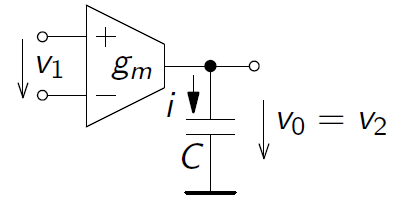
\includegraphics[scale=0.5]{otaintegrator.png}
\caption{OTA integrátor \cite{3}}
\end{figure}
Toto zapojení integrátoru s uzemněným kondenzátorem se označuje jako OTA-C. Ztrátový integrátor lze utvořit připojením paralelního rezistoru R, což vede na dolní propust 1. řádu s mezním kmitočtem RC. Toto je ekvivalentní se sériovým zapojením dalšího OTA se zápornou zpětnou vazbou. Rozdíl mezi ideálním a ztrátovým integrátorem lze pozorovat i v modulové charakteristice - pro ztrátový je konstantní a pak teprve lineárně klesá se sklonem -20 dB/dek.
\section{Integrované obvody s OTA zesilovači}
Integrované obvody se vyrábí buď s jedním nebo dvěma zesilovači v pouzdře. Varianty s jedním operačním zesilovačem jsou např. OPA615, OPA860 a novější OPA861 a jejich varianty. 
\renewcommand{\arraystretch}{1.5}
\begin{table}[H]
\scalebox{0.9}{%
  \begin{tabular}{ | c | >{\centering\arraybackslash}p{2cm}| >{\centering\arraybackslash}p{1.5cm} | >{\centering\arraybackslash}p{1.5cm} | >{\centering\arraybackslash}p{1.25cm} | >{\centering\arraybackslash}p{1.5cm} | >{\centering\arraybackslash}p{1.75cm} | >{\centering\arraybackslash}p{2cm} | >{\centering\arraybackslash}p{1.75cm} |}
    \hline
      & GBP - Gain Bandwidth Product & SR - Slew Rate & Output Current per Channel & $I_b$ - Input Bias Current & $V_{os}$ - Input Offset Voltage & Operating Supply Current & Forward Transconductance Min & Supply Voltage\\ \hline
    OPA615 & 710 MHz & 2.5 kV/$\mu$s & 5 mA & 3 $\mu$A & 40 mV & 13 mA & 65 mA/V & 8-12.4 V \\ \hline
    OPA860 & 470 MHz & 3.5 kV/$\mu$s & 15 mA & 5 $\mu$A & 12 mV & 11.2 mA & 80 mA/V & 5-13 V \\ \hline
    OPA861 & 400 MHz & 900 V/$\mu$s & 15 mA & 1 $\mu$A & 12 mV & 5.4 mA & 65 mA/V & 4-12.6 V  \\
    \hline
  \end{tabular}}
  \caption{\label{tab:Porovnání IO s jedním transkonduktančním OZ }Porovnání IO s jedním transkonduktančním OZ  \cite{4}}
  \end{table}
\noindent Všechny součástky s jedním OZ mají velkou šířku pásma (v řádech stovek MHz), cenově vychází na 75-280 Kč. Pro realizaci dolní propusti byly zvoleny vhodnější součástky s dvěma OZ - srovnání níže.
\begin{center}
\begin{table}[H]
\scalebox{0.9}{%
  \begin{tabular}{ | c | >{\centering\arraybackslash}p{2cm}| >{\centering\arraybackslash}p{1.5cm} | >{\centering\arraybackslash}p{1.5cm} | >{\centering\arraybackslash}p{1.25cm} | >{\centering\arraybackslash}p{1.5cm} | >{\centering\arraybackslash}p{1.75cm} | >{\centering\arraybackslash}p{2cm} | >{\centering\arraybackslash}p{1.75cm} |}
    \hline
      & GBP - Gain Bandwidth Product & SR  - Slew Rate & Output Current per Channel & $I_b$ - Input Bias Current & $V_{os}$ - Input Offset Voltage & Operating Supply Current & Forward Transconductance - Min & Supply Voltage\\ \hline
    LM13700 & 2 MHz & 50 V/$\mu$s & 650 $\mu$A & 5 $\mu$A & 4 mV & 1.3 mA & 6700 $\mu$S & 10-36 V \\ \hline
    NE5517 & 2 MHz & 50 V/$\mu$s & 650 $\mu$A & 5 $\mu$A & 5 mV & 2.6 mA & 5400 $\mu$S & 4-44 V \\ \hline
    AU5517 & 2 MHz & 50 V/$\mu$s & 650 $\mu$A & 5 $\mu$A & 5 mV & 2.6 mA & 5400 $\mu$S & 4-44 V  \\ \hline
    NJM13600 & 2 MHz & 50 V/$\mu$s & 650 $\mu$A & 5 $\mu$A & 5 mV & 2.6 mA & 6700 $\mu$S & 36 V  \\ \hline
    NJM13700 & 2 MHz & 50 V/$\mu$s & 650 $\mu$A & 5 $\mu$A & 4 mV & 2.6 mA & 6700 $\mu$S & 36 V  \\ \hline
  \end{tabular}}
  \caption{\label{tab:Porovnání IO s jedním transkonduktančním OZ}Porovnání IO s dvěma transkonduktančními OZ \cite{4}}
  \end{table}
\end{center}
\noindent Integrované obvody s dvěma OZ v pouzdře mají užší šířku pásma (2 MHz), menší rychlost přeběhu (50 V/$\mu$s), mnohem menší výstupní proud (650 $\mu$A) i offset vstupního napětí a operují při cca 4x nižších proudech. Cenové rozpětí je 25-65 Kč. Pro účely realizace filtru byla zvolena součástka LM13700M. 
\begin{figure}[H]
\centering
\includegraphics[scale=0.6]{image6.png}
\caption{Konfigurace pinů na LM13700M \cite{5}}
\end{figure}
\noindent Vnitřní zapojení LM13700 na obrázku 6 obsahuje symetrický rozdílový stupeň (tranzistory Q4, Q5), který je napájen řízeným zdrojem proudu s tranzistorem Q2. Dvojice diod a tranzistorů tvoří proudová zrcadla.
\begin{figure}[H]
\centering
\includegraphics[scale=0.25]{image5.png}
\caption{Schéma transkonduktančního zesilovače \cite{6}}
\end{figure}
\section{Dolní propust 2. řádu - teoretické odvození}
Využitím záporné zpětné vazby z výstupu a zapojením OTA zesilovačů sériově jako dva integrátory, byl obdržen dolnopropustní filtr 2. řádu.
\begin{figure}[H]
\centering
\includegraphics[scale=0.8]{image11.png}
\caption{Schéma s dvěma integrátory a zpětnou vazbou pro simulaci bikvadu \cite{7}}
\end{figure}
\begin{figure}[H]
\centering
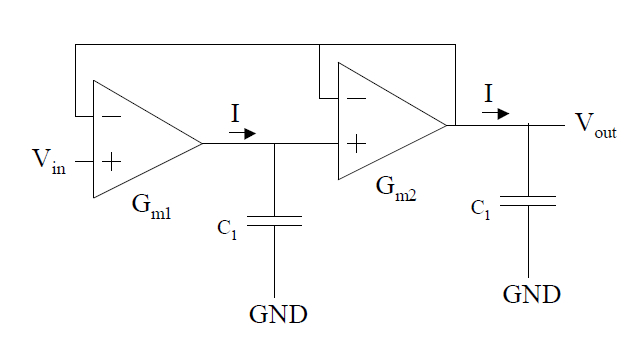
\includegraphics[scale=0.5]{zapojeni.png}
\caption{Dolní propust 2. řádu s OTA \cite{8}}
\end{figure}
\noindent Náhradní obvod, ze kterého bude spočítána přenosová funkce, popisuje obrázek 9.
\begin{figure}[H]
\centering
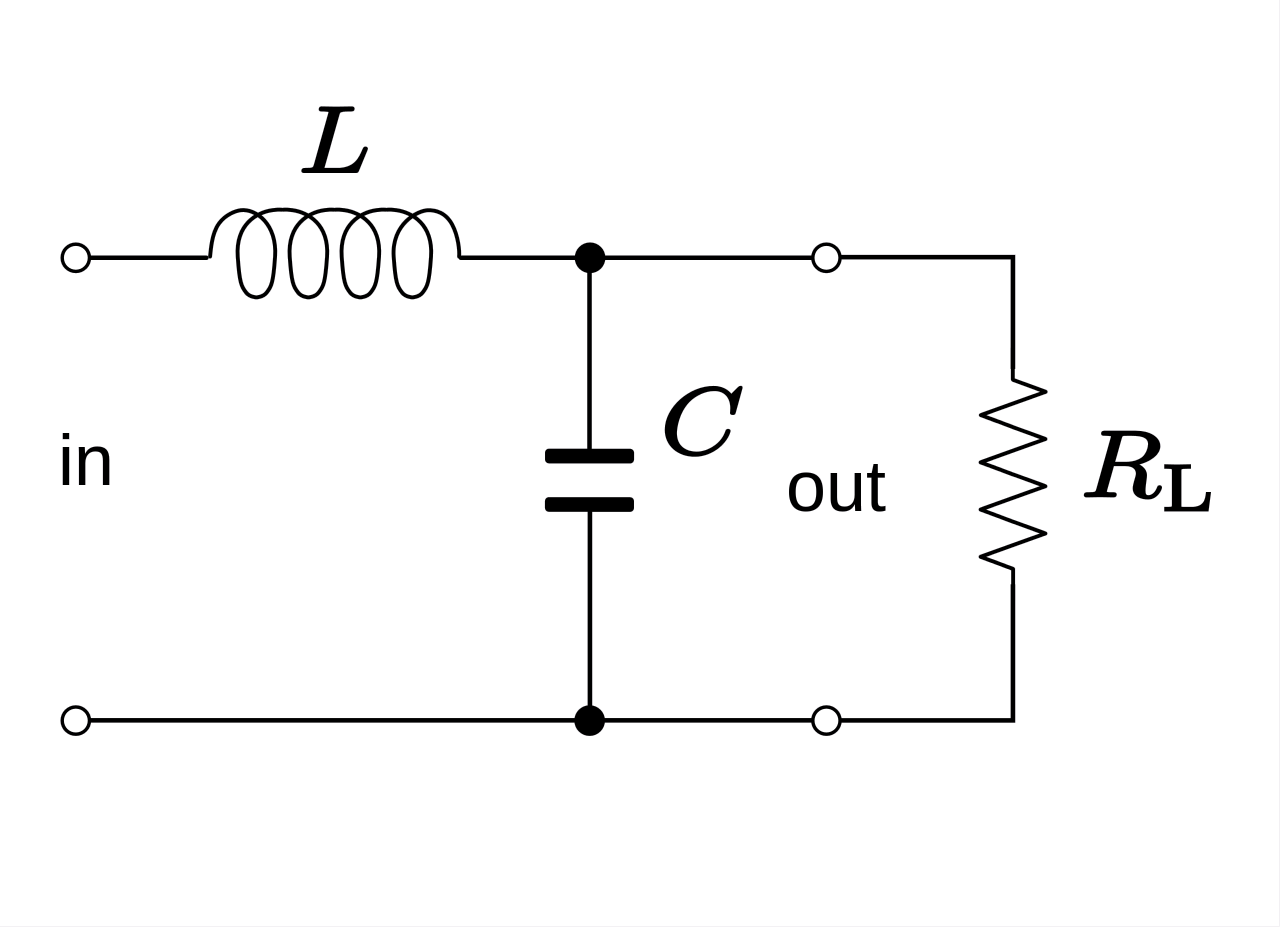
\includegraphics[scale=0.2]{RLC_low-pass.png}
\caption{Dolní propust 2. řádu (RLC obvod) \cite{9}}
\end{figure}
\noindent Přenos obvodu byl vyjádřen jako
\begin{align}
H(s) = \frac{U_{out}}{U_{in}} = \frac{Z_2}{Z_1},
\end{align}
kde $Z_1 = sL$ a $Z_2 = \frac{\frac{R}{sC}}{R + \frac{1}{sC}}$. Tedy
\begin{align}
H(s) = \frac{\frac{\frac{R}{sC}}{R + \frac{1}{sC}}}{sL + \frac{\frac{R}{sC}}{R + \frac{1}{sC}}}.
\end{align}
Elementárními algebraickými úpravami a následným vynásobením členem $\frac{1}{LRC}$ byl získán výsledný přenos.
\begin{align}
H(s) = \frac{R}{s^2LRC + sL + R} = \frac{\frac{1}{LC}}{s^2 + \frac{s}{RC} + \frac{1}{LC}}.
\end{align}
\noindent Pro ideální OTA zesilovač (vstupní i výstupní impedance nulové) je možno odpor nahradit obvodem na obrázku 10 a to hodnotou
\begin{align}
R_{in} = \frac{1}{g_{m1}},
\end{align}
kde $g_{m1}$ označuje transkonduktanci zesilovače. Prohození invertujícího a neinvertujícího vstupu vede na opačnou polaritu.
\begin{figure}[H]
\centering
\includegraphics[scale=0.7]{image10.png}
\caption{Obvod pro simulaci uzemněného rezistoru \cite{7}}
\end{figure}
\noindent Pro uzemněnou indukčnosti o impedanci $Z_L = \frac{1}{sC}$ byl použit obvod na obrázku 11. Vyjádřením napětí a proudů v obvodu bylo získáno 
\begin{align}
V_C &= \frac{g_{m1}}{sC}V_1 \\
I_1 &= g_{m2}V_C = \frac{g_{m1}g_{m2}}{sC}V_1.
\end{align}
Výsledná indukčnost - impedance vstupu byla vyjádřena vztahem (11).
\begin{align}
Z_{in}(s) = \frac{V_1}{I_1} = s\frac{C}{g_{m1}g_{m2}}
\end{align}
\begin{figure}[H]
\centering
\includegraphics[scale=1]{image12.png}
\caption{Obvod pro simulaci uzemněné indukčnosti pro $g_{m1} = g_{m2}$\cite{7}}
\end{figure}
\noindent Pro obdržení plovoucí indukčnosti je nutné zrušit uzemnění invertujícího vstupu prvního OTA zesilovače a zachovat $I_1 = I_2$ (obrázek 12). Přidáním další transkonduktance $g_{m3}$ bylo získáno
\begin{align}
V_C = \frac{g_{m1}}{sC}(V_1 - V_2).
\end{align}
Pro proudy $I_1, I_3$ platí
\begin{align}
I_1 &= g_{m2}V_C = \frac{g_{m1}g_{m2}}{sC}(V_1 - V_2)\\
I_3 &= g_{m3}V_C = \frac{g_{m1}g_{m3}}{sC}(V_1 - V_2).
\end{align}
Pro ekvivalentní transkonduktance $g_{m1} = g_{m2} = g_{m3}$ byl obdržen plovoucí induktor o hodnotě
\begin{align}
L = \frac{C}{g_{m1}g_{m2}}.
\end{align}
\begin{figure}[H]
\centering
\includegraphics[scale=0.6]{image13.png}
\caption{Obvod pro simulaci neuzemněné indukčnosti pro $g_{m1} = g_{m2} = g_{m3}$\cite{7}}
\end{figure}
\noindent Nyní je možno za odpor a indukčnost dosadit do vztahu (7). Byly uvažovány kapacitory o stejné hodnotě C.
\begin{align}
H(s) = \frac{\frac{1}{\frac{C^2}{g_{m1}g_{m2}}}}{s^2 + \frac{s}{\frac{C}{g_{m2}}} + \frac{1}{\frac{C^2}{g_{m1}g_{m2}}}} = \frac{\frac{g_{m1}g_{m2}}{C^2}}{s^2 + \frac{sg_{m2}}{C} + \frac{g_{m1}g_{m2}}{C^2}} = \frac{g_{m1}g_{m2}}{s^2C^2 + sg_{m2}C + g_{m1}g_{m2}}.
\end{align}
Porovnáním jmenovatele se jmenovatelem přenosu filtru 2. řádu byl obdržen vztah
\begin{align}
s^2 + s\frac{\omega _0}{Q} + \omega _0^2 &= s^2C^2 + sg_{m2}C + g_{m1}g_{m2}\\
s^2 + s\frac{\omega _0}{Q} + \omega _0^2 &= s^2 + \frac{sg_{m2}}{C} + \frac{g_{m1}g_{m2}}{C^2}.
\end{align}
Z tohoto vztahu byl vyjádřen mezní kmitočet jako 
\begin{align}
\omega _0^2 &= \frac{g_{m1}g_{m2}}{C^2} \\
\omega _0 &= \sqrt{\frac{g_{m1}g_{m2}}{C^2}}
\end{align}
a činitel jakosti dosazením za $\omega _0$
\begin{align}
Q = \frac{\omega _0}{\frac{g_{m2}}{C}} = \sqrt{\frac{g_{m1}}{g_{m2}}}.
\end{align}
\section{Dolní propust 2. řádu - simulace}
Zapojení dvou transkonduktančních zesilovačů v sérii jako integrátorů vede na dolní propust druhého řádu. Symetrické napájení operačních zesilovačů $V_{DD},V_{SS} = \pm 15$ V a vstupní externí proud $I_{ABC} = 500$ $\mu$A jsou zvoleny podle dokumentace k integrovanému obvodu LM13700M. Regulací vstupního proudu je ovlivňován pracovní bod obvodu, tzn. hodnota mezního kmitočtu. Při externím proudu $I_{ABC} \in$ $<5$ $\mu$A ; 500 $\mu$A> je výrobcem garantováno minimální výstupní napětí $U_{OUT} = \pm 12$ V, standardně $V_{peak 1} = 14.2$ V a $V_{peak 2} = -14.4$ V. Při výstupním napětí v tomto intervalu je šum vzhledem k signálu zanedbatelný a nezkreslí výsledky simulace.\\
Volbou mezního kmitočtu $\omega _0 = 100$ kHz a dosazením $g_m = 9600$ $\mu$S do vztahu (21) byly obdrženy hodnoty kondenzátorů $C = C_1 = C_2 = 120$ nF.
\begin{figure}[H]
\centering
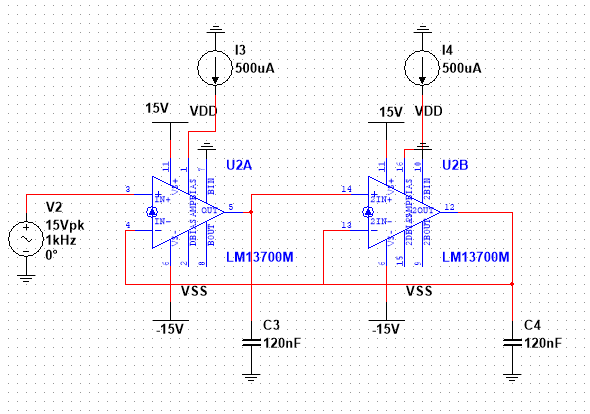
\includegraphics[scale=0.75]{lowpasszapojeni.png}
\caption{Schéma zapojení dolní propusti 2. řádu s LM13700M}
\end{figure}
\begin{figure}[H]
\centering
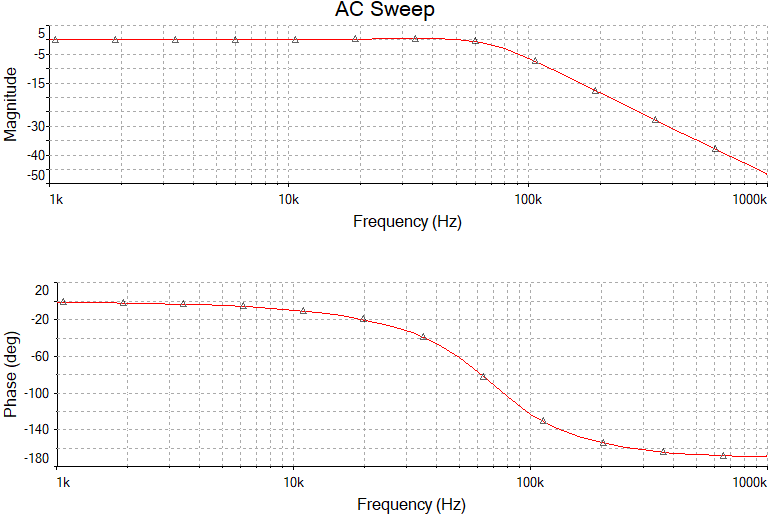
\includegraphics[scale=0.75]{lowpass2.png}
\caption{Amplitudová a fázová charakteristika dolní propusti 2. řádu}
\end{figure}
\section{Pásmová propust}
Umístěním dvou kapacitorů a dvou rezistorů do základního obvodu byla obdržena pásmová propust. Napájecí napětí a vstupní klidový proud byl zvolen z dokumentace obdobně jako pro zapojení dolní propusti.
\begin{figure}[H]
\centering
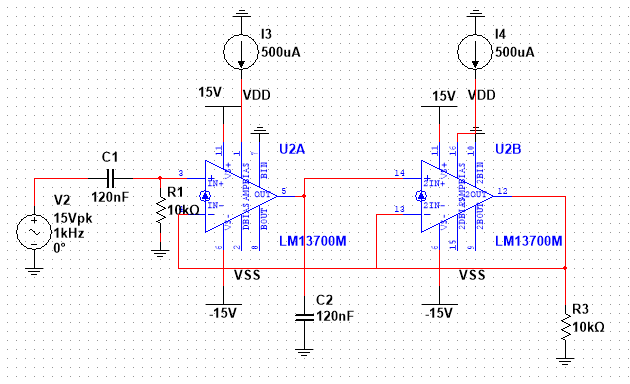
\includegraphics[scale=0.75]{bandpasszapojeni.png}
\caption{Schéma zapojení pásmové propusti s LM13700M}
\end{figure}
\begin{figure}[H]
\centering
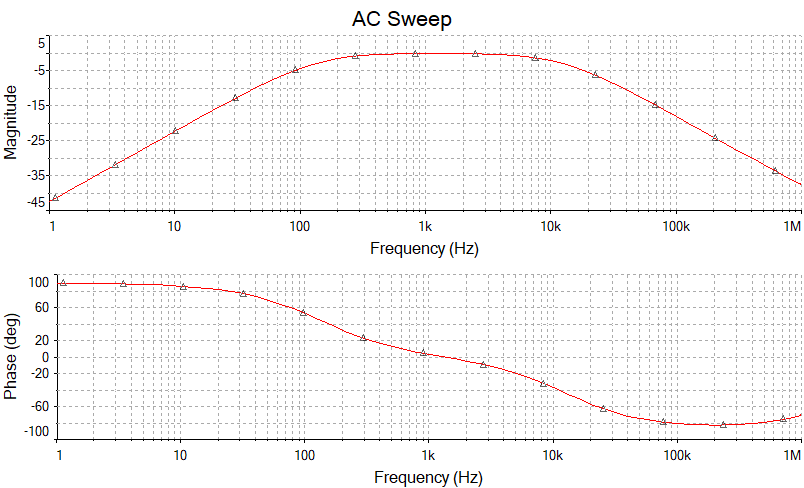
\includegraphics[scale=0.75]{bandpass2.png}
\caption{Amplitudová a fázová charakteristika pásmové propusti}
\end{figure}
\noindent Pokud bude požadována úzká šířka pásma, k realizaci bude postačovat obvod s dvěma kapacitory. Volbě propustného pásma $\omega _0 = 12-14$ kHz odpovídá modulová charakteristika na obrázku 18. Oproti předchozímu zapojení byl obdržen vyšší činitel jakosti (def.: činitel jakosti $Q = \frac{1}{B}$, kde B je šířka pásma definovaná rozdílem kmitočtů, při kterých klesne přenos cca o -3dB).
\begin{figure}[H]
\centering
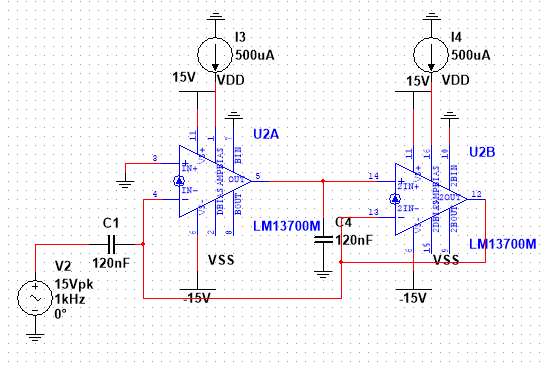
\includegraphics[scale=0.75]{uzkybpschema.png}
\caption{Schéma zapojení pásmové propusti s užší šířkou propustného pásma (LM13700M)}
\end{figure}
\begin{figure}[H]
\centering
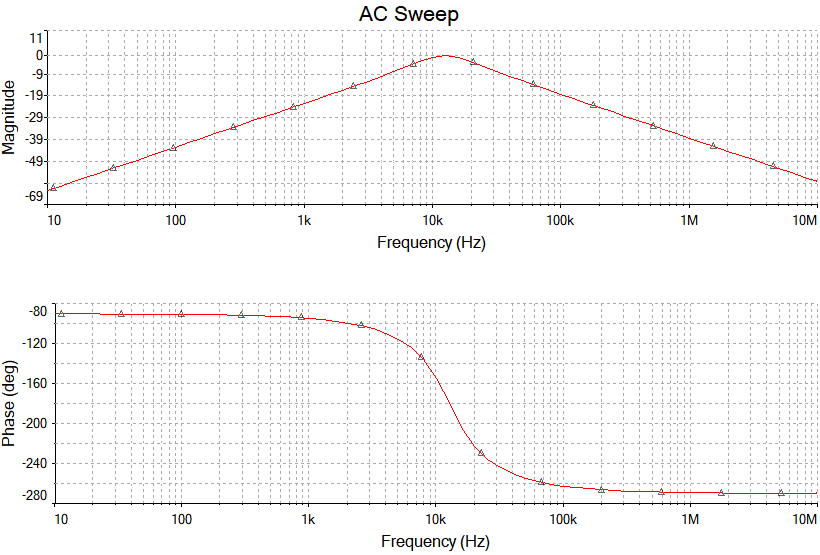
\includegraphics[scale=0.75]{uzkybp.png}
\caption{Amplitudová a fázová charakteristika pásmové propusti s užší šířkou propustného pásma}
\end{figure}
\section{Dolní propust vyšších řádů - simulace}
Kaskádním zapojením dolní propusti ze sekce 5 byly obdrženy následující výsledky. Byl obdržen filtr 3. řádu s poklesem -60 dB/dek.
\begin{figure}[H]
\centering
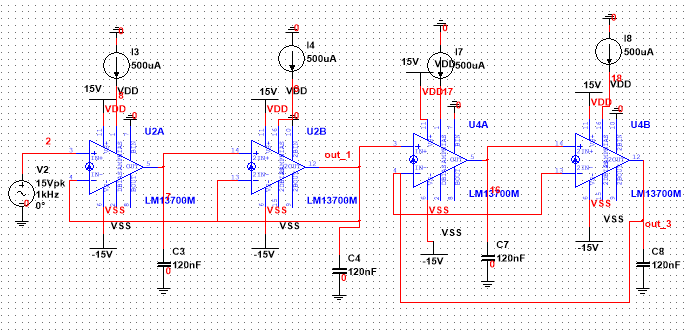
\includegraphics[scale=0.75]{kaskadneschema.png}
\caption{Schéma kaskádního zapojení dolní propusti}
\end{figure}
\begin{figure}[H]
\centering
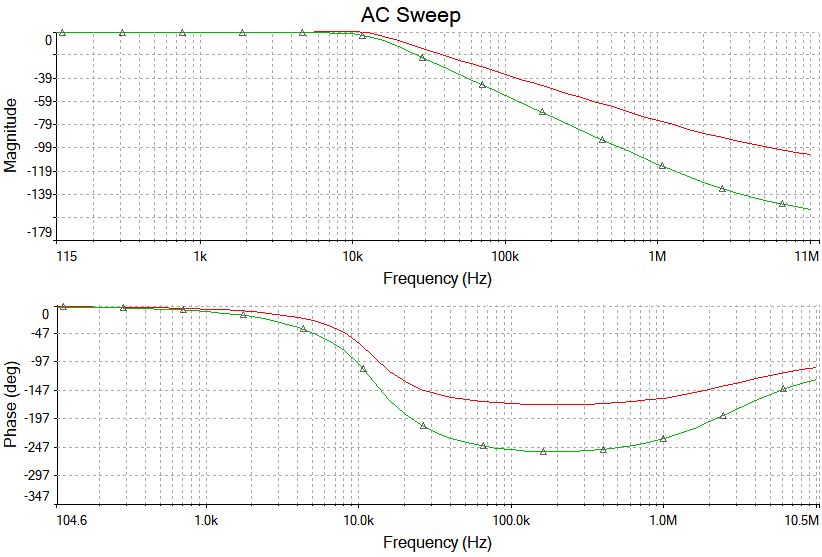
\includegraphics[scale=0.75]{kaskadne1.png}
\caption{Amplitudová a fázová charakteristika káskádního zapojení dolní propusti}
\end{figure}
\begin{thebibliography}{999}
\bibitem{1}
HOSPODKA, Jiří. \textit{Úvod do syntézy kmitočtových filtrů} [online]. Praha, 2018 [cit. 2019-03-30]. Dostupné z: \url{https://moodle.fel.cvut.cz/course/view.php?id=2670}. Přednáška. ČVUT FEL. Slide 23/24.
\bibitem{2}
MICHAL, Vratislav. \textit{Vybrané vlastnosti obvodů pracujících v proudovém módu a napěťovém módu} [online]. Brno, 2017 [cit. 2019-03-30]. Dostupné z: \url{https://docplayer.cz/43256146-Vybrane-vlastnosti-obvodu-pracujicich-v-proudovem-modu-a-napetovem-modu.html}. Článek. Brno University of Technology. Strana 5/6.
\bibitem{3}
HOSPODKA, Jiří. \textit{Úvod do analogových filtrů} [online]. Praha, 2018 [cit. 2019-03-30]. Dostupné z: \url{https://moodle.fel.cvut.cz/course/view.php?id=1434}. Přednáška. ČVUT FEL. Slide 24/41.
\bibitem{4}
\textit{Transconductance Amplifiers} [online]. 2019 [cit. 2019-03-30]. Dostupné z: \url{https://cz.mouser.com/Semiconductors/Integrated-Circuits-ICs/Amplifier-ICs/Transconductance-Amplifiers/_/N-6j73l?P=1y95od0}
\bibitem{5}
LM13700: Dual Operational Transconductance Amplifiers With Linearizing Diodes and Buffers. In: \textit{Texas Instruments} [online]. Dallas, Texas: Texas Instruments Incorporated, 2018 [cit. 2019-03-30]. Dostupné z: \url{www.ti.com/lit/ds/symlink/lm13700.pdf} Strana 1/37.
\bibitem{6}
ZUMCHAK, Gene.  \textit{A Short Discussion of the Operational Transconductance Amplifier (OTA)}. Synthesizer DIY pages of René Schmitz [online]. 1999 [cit. 2019-03-30]. Dostupné z: \url{https://www.schmitzbits.de/ota3080.html} Obrázek 5.
\bibitem{7}
SCHAUMANN, Rolf a Mac E. Van VALKENBURG. \textit{Design of Analog Filters}. New York: Oxford University Press, 2001. ISBN 0195118774. Pořadě obrázek 5-33 b), 4-13, 4-36 a), b).
\bibitem{8}
HASLER, Paul. \textit{Basics of Transconductance – Capacitance Filters}. In: Integrated Computational Electronics Laboratory (ICE) [online]. 2019 [cit. 2019-03-30]. Dostupné z: \url{hasler.ece.gatech.edu/Courses/ECE6414/Unit3/gmCFilter01.pdf} Slide 21/27.
\bibitem{9}
Low-pass filter. In: \textit{Wikipedia: the free encyclopedia} [online]. San Francisco (CA): Wikimedia Foundation, 2001- [cit. 2019-03-30]. Dostupné z: \url{https://en.wikipedia.org/wiki/Low-pass_filter}
\end{thebibliography}
\end{document}